\section{The Quantum Adder-Subtractor}

In this section we are going to construct using the Qiskit SDK the quantum cirucit of the Adder-Subtractor. This will
be the final version of the integer addition-subtraction unit of the Quantum Arithmetic Logic Unit.

\subsection{Analysing the diagram and logic of the Adder-Subtractor circuit}

The Adder-Subtractor circuit, is a digital circuit that computes the sum or the difference of two $n$-bit inputs
and produces an $n$-bit sum or difference, denoted by $O$, and an carry-out overflow bit $C_{overflow}$. This
digital circuit is constructed using the Ripple Carry Adder circuit. As mentioned in Chapter 2, binary subtraction
can be implemented by addition if we take the 2s-complement of the subtrahend and sum it with the minuend. This
saves us from using two different circuits - it takes less logic gates to implement the two operations.

\begin{figure}[!ht]
    \centering
    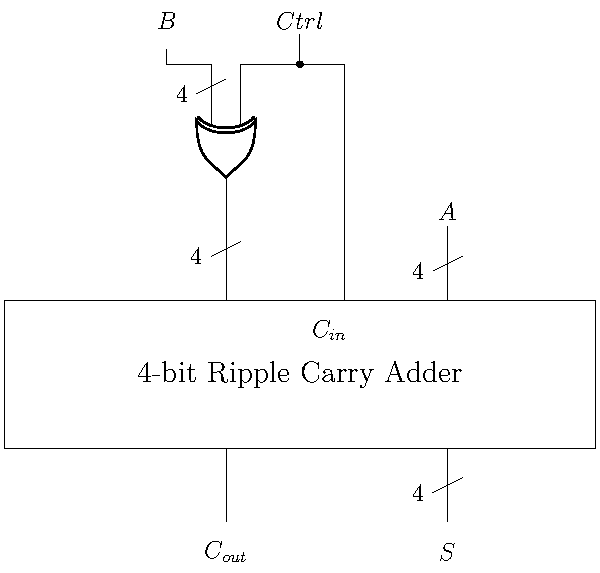
\includegraphics[height=6cm]{images/5_Implementation/classical_adder_subtractor.pdf}
    \caption{The diagram of the classical Adder-Subtractor circuit}
\end{figure}

The Adder-Subtractor works by having one extra wire, denoted as $CTRL$ in the diagram, that controls the mode
of the circuit: zero for addition and one for subtraction. We will skip the first mode because we have covered
that in the previous subsection. The more interesting part is the subtraction mode.

While in subtraction mode, input $B$ and $CTRL$ bit are XOR'ed together to produce the 1s-complement of $B \rightarrow B'$.
To get the 2s-complement, we need to add one to $B' + 1$. This can be done by supplying the $C_{in}$ input of the
4-bit Ripple Carry Adder with the $Ctrl$ wire.

To implement this quantum circuit we are going to need the $QRCA$ gate that we created on the previous subsection and
$n+1$ CNOT gates, so that we can take the 1s-complement of input $B$ and $C_{in_{0}}$. First we apply the CNOT gate, with
the control qubit set to $Ctrl$ and target each qubit of register $B$. We also do the same for the $C_{in_{0}}$ qubit.
Finally we apply the $QRCA$ - the quantum Ripple Carry Adder. This will transform register $C_{in}$ into the register $Out$
which essential stores either the summation or difference of input quantum registers $A$ and $B$.

\subsection{The Python3 implementation}

For this implementation we are going to use the Quantum Ripple Carry Adder, discussed in the previous section.
First, we are going to initialize all the apropriate registers, $A$ and $B$ which store the terms, $CTRL$ which
stores information about the mode of the unit, $C_{in}$ which is either initialized to all-zeros ($\ket{0^{\otimes n}}$)
or all-zeros except the LSB (least significant (qu)bit) which is set by $CTRL$.

\begin{listing}[!ht]
    \centering
    \begin{minted}{python3}
        from qiskit import QuantumCircuit, QuantumRegister

        ctrl = QuantumRegister(1, name="Ctrl")
        a = QuantumRegister(n, name="A")
        b = QuantumRegister(n, name="B")
        cin = QuantumRegister(n, name="Cin")
        cout = QuantumRegister(1, name="Cout")
        circuit = QuantumCircuit(ctrl, a, b, cin, o)
    \end{minted}
    \caption{Initialization of the Adder-Subtractor circuit}
\end{listing}

Next we are going to invert all qubits of register $B$ by applying the CNOT gate to each qubit controlled by 1-qubit
register $CTRL$. We also invert the LSB of register $C_{in}$ to acquire the 2s-complement of register $B$. After that,
we apply the QRCA gate and finally un-compute reigster $B$.

\begin{listing}[!ht]
    \centering
    \begin{minted}{python3}
        for i in range(n):
            circuit.cx(ctrl, b[i])
        circuit.cx(ctrl, cin[0])
        circuit.append(rca, (a[:] + b[:] + cin[:] + o[:]))
        for i in reversed(range(n)):
            circuit.cx(ctrl, b[i])
    \end{minted}
    \caption{Step-by-step instructions of the quantum Adder-Subtractor circuit}
\end{listing}

\begin{figure}[!ht]
    \centering
    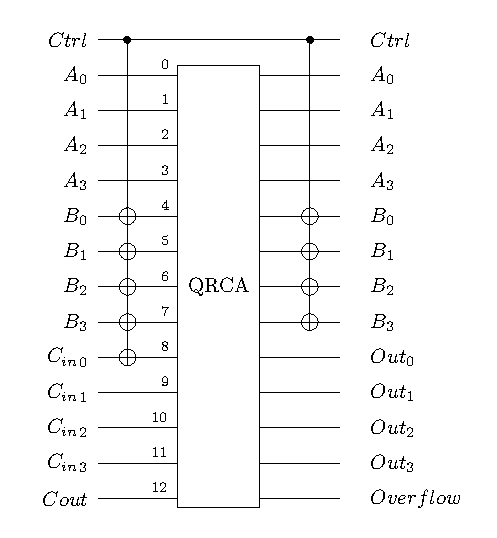
\includegraphics{images/5_Implementation/quantum_adder_subtractor.pdf}
    \caption{The diagram of the quantum Adder-Subtractor circuit}
\end{figure}